%! Author = krystian
%! Date = 08.03.2020

% Preamble
\documentclass[11pt]{article}
\usepackage{graphicx}
\usepackage[export]{adjustbox}
\usepackage{float}
\author{Krystian \.Zyci\'nski}
\title{Sprawozdanie z mierzenia opóźnienia i przepustowości w klastrze}
\date{\the\year}

% Packages

% Document
\begin{document}
    \maketitle
    \clearpage
    \section{Wstęp}\label{sec:1}
    \subsection{Cel projektu}
    Celem projektu było zapoznanie z komunikacją P2P w MPI i zmierzenie za jej pomocą opóźnienia oraz
    przepustowości połączeń w klastrze.
    Należało przetestować dwa różne typy komunikacji, dokonać odpowiednich
    pomiarów i storzyć na ich podstawie wykresy.
    Dodatkowo wyniki powinny uwzględniać następujące konfiguracje:
    \begin{enumerate}
        \item Komunikacja na 1 nodzie (pamięć współdzielona),
        \item Komunikacja na 1 nodzie (bez pamięci współdzielonej, przez sieć),
        \item Komunikacja między 2 nodami na tym samym hoście fizycznym (przez sieć),
        \item Komunikacja między 2 nodami na różnych hostach fizycznych (przez sieć).
    \end{enumerate}
    \subsection{Sposób wykonania}
    Do implementacji algorytmów został wykorzystany język Python oraz biblioteka \texttt{mpi4py}.
    Przy mierzeniu przepustowości zostały wykorzystane pythonowe \textit{bytearray} o odpowiednich rozmiarach.
    Do dokładnego zmierzenia czasu zostały wykorzystane funkcje z MPI, mianowicie \texttt{MPI\_Barrier} do
    zapewnienia, że oba procesy są rozpoczęte, oraz \texttt{MPI.Wtime()} do zmierzenia samego czasu.
    Wyniki zostały zapisywane w plikach \textit{.csv}.
    Programy zostały uruchomione w następujących konfiguracjach:
    \begin{enumerate}
        \item vnode-02
        \item vnode-02
        \item vnode-02, vnode-03
        \item vnode-06, vnode-09
    \end{enumerate}
    Przed uruchomieniem każdej konfiguracji klastry zostały sprawdzone z użyciem funkcji \textit{htop}, aby
    uniknąć dokonania obliczeń na obciążonym środowisku.

    Każdy eksperyment został przeprowadzony 20 razy z różnymi wartościami parametrów.
    Eksperymenty polegały na wymianie 50000 wiadomości między procesami z różnym rozmiarem wysyłanych danych
    (rozmiary widać na wykresach).

    Do wykonania eksperymentu wybrałem metodę wysyłania synchronicznego oraz metodę wysyłania bufora.

    \clearpage
    \section{Wyniki obliczeń}
    \subsection{Komunikacja na 1 nodzie---pamięć współdzielona}
    Jak można się spodziewać pamięć współdzielona daje najlepsze możliwe rezultaty:

    \renewcommand{\figurename}{Wykres}
    \begin{figure}[H]
        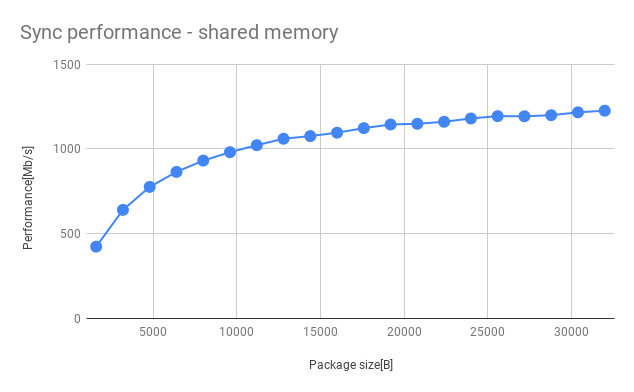
\includegraphics[width=1\textwidth,frame]{charts/Sync performance - shared memory.png}
        \caption{Przepustowość metody sync dla pamięci współdzielonej}
        \label{fig:sync-shared-performance}
    \end{figure}
    \begin{figure}[H]
        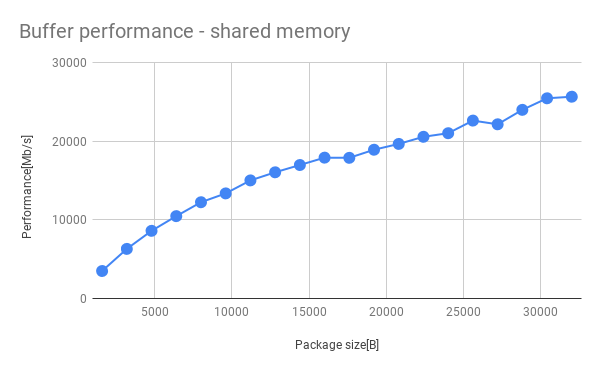
\includegraphics[width=1\textwidth,frame]{charts/Buffer performance - shared memory.png}
        \caption{Przepustowość metody buforowania dla pamięci współdzielonej}
        \label{fig:buff-shared-performance}
    \end{figure}


    \begin{figure}[H]
        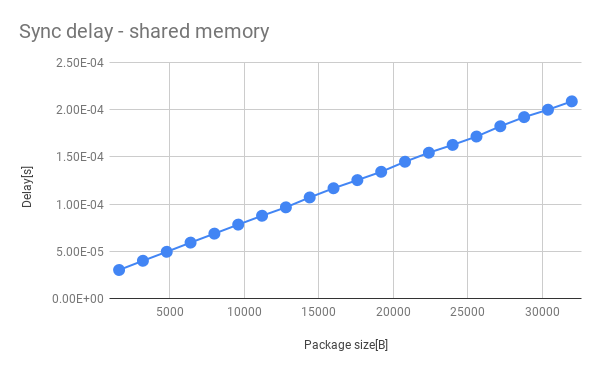
\includegraphics[width=1\textwidth,frame]{charts/Sync-delay-shared-memory.png}
        \caption{Opóźnienie metody sync dla pamięci współdzielonej}
        \label{fig:sync-shared-delay}
    \end{figure}
    \begin{figure}[H]
        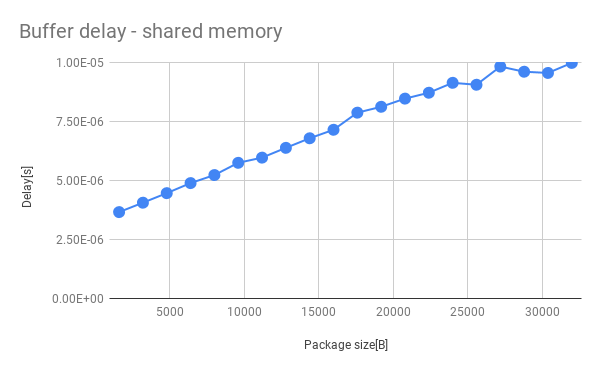
\includegraphics[width=1\textwidth,frame]{charts/Buffer delay - shared memory.png}
        \caption{Opóźnienie metody buforowania dla pamięci współdzielonej}
        \label{fig:buff-shared-delay}
    \end{figure}

    W obu przypadkach wraz ze wzrostem rozmiaru paczki wysyłanych danych można zaobserwować wzrost
    przepustowości oraz opóźnienia.
    Widać także wyższość wysyłania buforów danych---przesyłanie jest kilkadziesiąt razy szybsze przy znacznie mniejszym
    opóźnieniu dla pojedyńczej operacji.

    \subsection{Komunikacja na 1 nodzie---przez sieć)}

    Podczas uruchamiania testu w tej konfiguracji, można się spodziewać wyników dużo gorszych niż w przypadku
    pamięci współdzielonej, porównywalnych do kolejnych testów komunikacji przez sieć.
    Jednak otrzymywane wyniki były wręcz identyczne co przy pamięci współdzielonej, mimo wielu prób uruchomienia
    na różne sposoby (między innymi działająca przy implementacji w C flaga \texttt{MPIR\_CVAR\_CH3\_NOLOCAL}).
    W związku z tym można wywnioskować, że \texttt{mpi4py} nie umożliwia użytkownikom uruchomienia procesów
    komunikujących się przez sieć kiedy znajdują się na tym samym nodzie.

    \subsection{Komunikacja między 2 nodami na tym samym hoście fizycznym---przez sieć}
    Przy komunikacji przez sieć można zauważyć kilkukrotny spadek wydajności:
    \begin{figure}[H]
        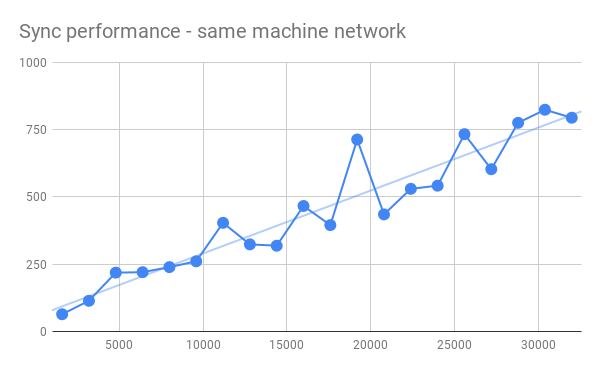
\includegraphics[width=1\textwidth,frame]{charts/Sync performance - same machine network.png}
        \caption{Przepustowość metody sync dla tego samego hosta fizycznego}
        \label{fig:sync-same-performance}
    \end{figure}
    Na wykresie widać wahania, można przypuszczać że są one spowodowane narzutem na sieć AGH.
    Jest także zaznaczona linia trendu która jednoznacznie wskazuje na wzrost wydajności wraz ze wzrostem rozmiaru paczki.

    \begin{figure}[H]
        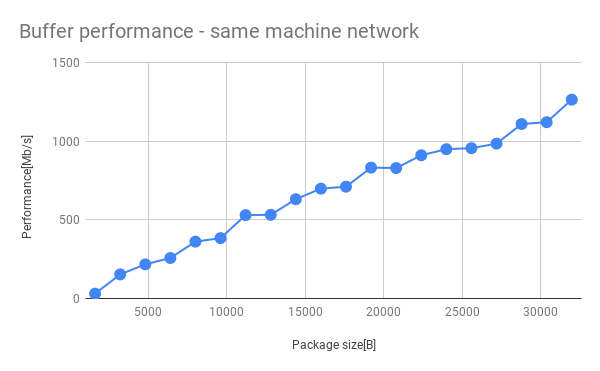
\includegraphics[width=1\textwidth,frame]{charts/Buffer performance - same machine network.png}
        \caption{Przepustowość metody buforowania dla tego samego hosta fizycznego}
        \label{fig:buff-same-performance}
    \end{figure}


    \begin{figure}[H]
        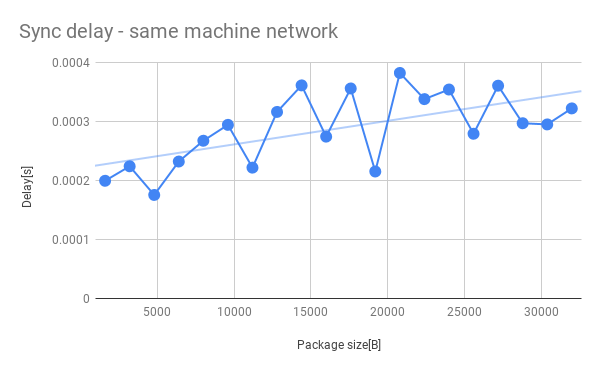
\includegraphics[width=1\textwidth,frame]{charts/Sync delay - same machine network.png}
        \caption{Opóźnienie metody sync dla tego samego hosta fizycznego}
        \label{fig:sync-same-delay}
    \end{figure}
    \begin{figure}[H]
        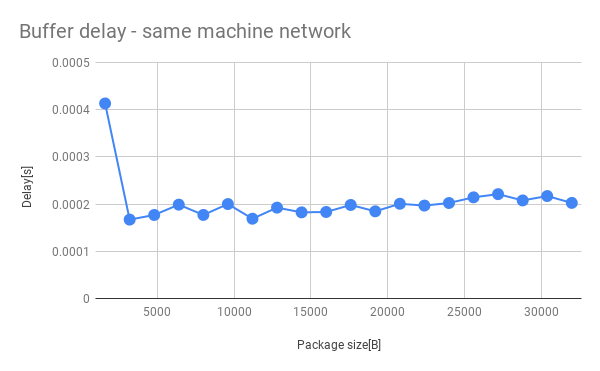
\includegraphics[width=1\textwidth,frame]{charts/Buffer delay - same machine network.png}
        \caption{Opóźnienie metody buforowania dla tego samego hosta fizycznego}
        \label{fig:buff-same-delay}
    \end{figure}

    Widać także zmiane w opóźnieniach---przy metodzie sync nie zmienia się ono tak gwałtownie jak w przypadku
    pamięci współdzielonej, a przy przetwarzaniu buforowym jest ono wręcz niezmienne (poza pierwszym pomiarem,
    który można uznać za błędny).

    Ponadto widać także zbliżenie się metody buforowania do synchronicznej---różnica w przepustowości nie jest już tak ogromna.


    \subsection{Komunikacja między 2 nodami na różnych hostach fizycznych---przez sieć}

    W tym eksperymencie można się spodziewać jeszcze mniejszej wydajności, ze względu na dłuższą trasę, jaką muszą przebyć
    dane.

    \begin{figure}[H]
        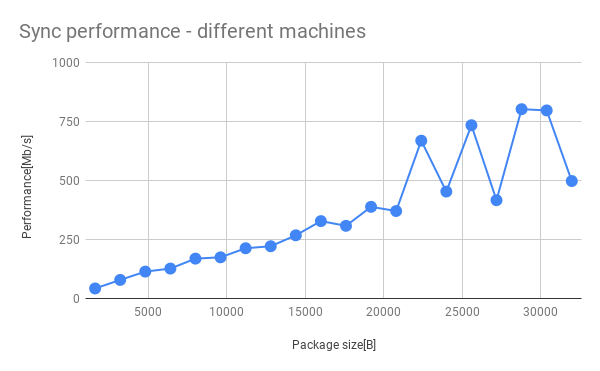
\includegraphics[width=1\textwidth,frame]{charts/Sync performance - different machines.png}
        \caption{Przepustowość metody sync dla różnych hostów fizycznych}
        \label{fig:sync-diff-performance}
    \end{figure}

    \begin{figure}[H]
        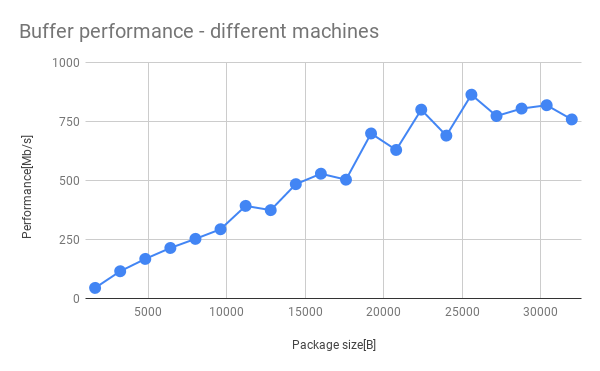
\includegraphics[width=1\textwidth,frame]{charts/Buffer performance - different machines.png}
        \caption{Przepustowość metody buforowania dla różnych hostów fizycznych}
        \label{fig:buff-diff-performance}
    \end{figure}

    Metoda sync ma porównywalne wyniki co na tej samej maszynie, jednak buforowanie ucierpiało jeszcze bardziej i osiąga
    niemal identyczne wyniki co sync.
    Widać także zachwianie się na wykresie metody synchronicznej---ponownie prawdopodobnym powodem jest narzut na sieć.

    \begin{figure}[H]
        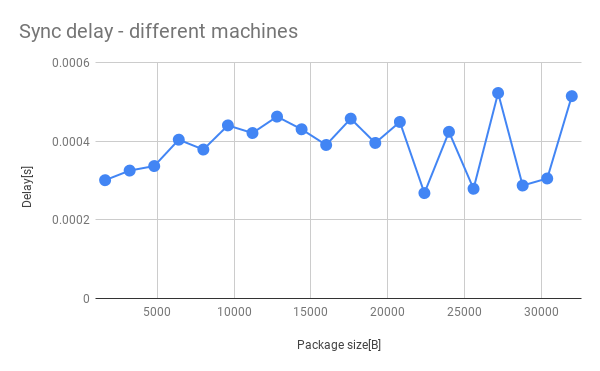
\includegraphics[width=1\textwidth,frame]{charts/Sync delay - different machines.png}
        \caption{Opóźnienie metody sync dla różnych hostów fizycznych}
        \label{fig:sync-diff-delay}
    \end{figure}
    \begin{figure}[H]
        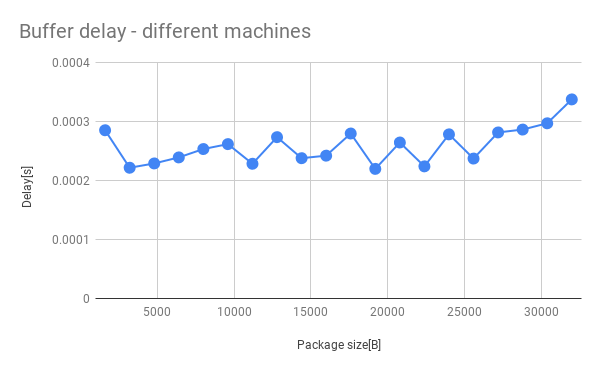
\includegraphics[width=1\textwidth,frame]{charts/Buffer delay - different machines.png}
        \caption{Opóźnienie metody buforowania dla różnych hostów fizycznych}
        \label{fig:buff-diff-delay}
    \end{figure}

    Zdecydowanie najwyższe jak dotąd opóźnienia, wyniki zgadzają się ze spodziewanymi.
    \clearpage
    \section{Wnioski}
    Jak widać najlepszą i najszybszą konfiguracją jest pamięć wpółdzielona.
    Na drugim miejscu prawdopodobnie znalazłaby się metoda komunikacji na jednym nodzie przez sieć, jednak
    doświadczenia nie udało się przeprowadzić.

    Najwolniejszą metodą były 2 różne hosty fizyczne---pakiety danych musiały przebyć najdłuższą drogę, na
    współdzielonych odcinkach.

    \subsection{Porównania konfiguracji}
    \subsubsection{Przepustowość}
    \begin{figure}[H]
        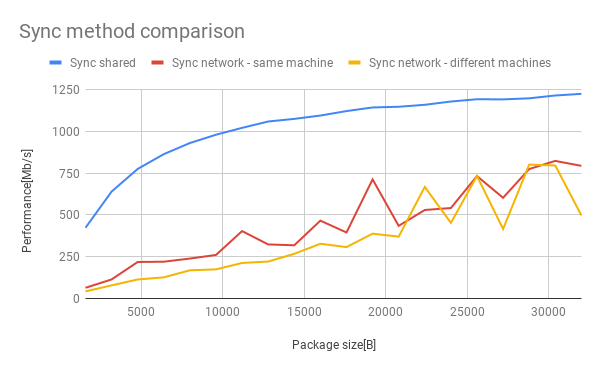
\includegraphics[width=1\textwidth,frame]{charts/Sync method comparison.png}
        \caption{Porównanie przepustowości dla metody synchronicznej}
        \label{fig:sync-comparison}
    \end{figure}

    Pamięć współdzielona jest kilka razy wydajniejsza niż porozstałe, nie ma także wahań na końcu, bo duże pakiety
    danych nie musiały na siebie czekać.

    \begin{figure}[H]
        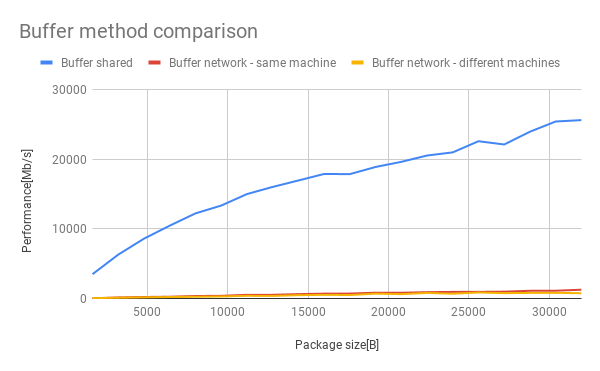
\includegraphics[width=1\textwidth,frame]{charts/Buffer method comparison.png}
        \caption{Porównanie przepustowości dla metody bufforowania}
        \label{fig:buffer-comparison}
    \end{figure}

    Jak widać w tej metodzie pamięć współdzielona nie pozostawia suchej nitki na konkurencji.
    Warto jednak przyjrzeć się samej komunikacji poprzez sieć:

    \begin{figure}[H]
        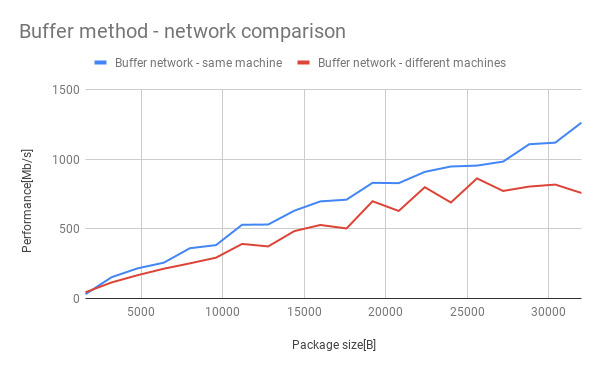
\includegraphics[width=1\textwidth,frame]{charts/Buffer method - network comparison.png}
        \caption{Porównanie przepustowości dla metody bufforowania---konfiguracje sieciowe}
        \label{fig:buffer-net-comparison}
    \end{figure}

    Sieć na tej samej maszynie pod koniec doświadczenia zaczęła się oddalać od konkurenta, można
    założyć że w miare zwiększania paczki ta różnica powiększałaby się jeszcze bardziej.

    \subsubsection{Opóźnienie}

    \begin{figure}[H]
        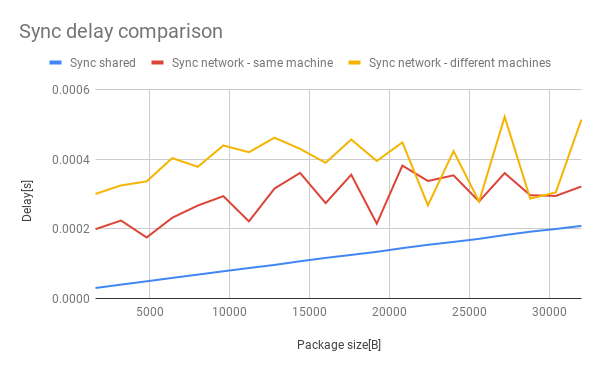
\includegraphics[width=1\textwidth,frame]{charts/Sync delay comparison.png}
        \caption{Porównanie opóźnienia dla metody synchronizacji}
        \label{fig:sync-delay-comparison}
    \end{figure}

    Pamięć współdzielona (jak można się było spodziewać) ma najmniejsze opóźnienia.
    Warto także zwrócić uwagę na zaburzenia związane z narzutem na sieć, szczególnie widoczne przy dużych paczkach.

    \begin{figure}[H]
        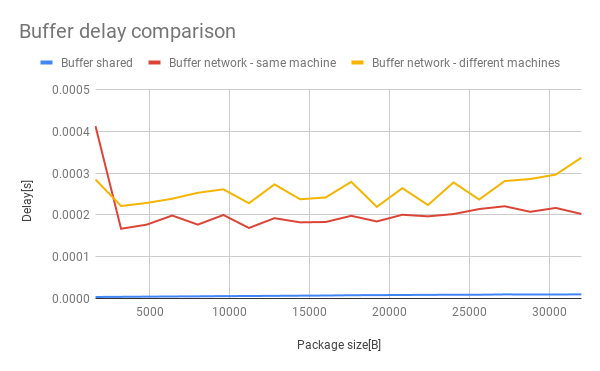
\includegraphics[width=1\textwidth,frame]{charts/Buffer delay comparison.png}
        \caption{Porównanie opóźnienia dla metody bufforowania}
        \label{fig:buffer-delay-comparison}
    \end{figure}

    Przy metodzie buforowania widać mniejsze wahania, lecz dużo większą różnicę w opóźnieniu przy przesyłaniu przez siec
    i przy pamięci współdzielonej.
\end{document}
